\documentclass[a4paper,12pt]{report}

\usepackage{cmap}
\usepackage[T2A]{fontenc}
\usepackage[utf8]{inputenc}
\usepackage[english,russian]{babel}
\usepackage{listings}
\usepackage{amsmath}
\usepackage{amsfonts}
\usepackage{float}
\usepackage{csquotes}
\usepackage{hyphenat}

% \usepackage{titlesec}
% \newcommand{\sectionbreak}{\clearpage}

\usepackage{graphicx}
\graphicspath{ {./images/} }

\usepackage{xcolor}
% \usepackage{courier}

\usepackage[
    backend=biber,
    style=alphabetic,
    sorting=ynt
]{biblatex}
\addbibresource{resources.bib}

\definecolor{buzzlightyear}{HTML}{8757A5}
\definecolor{grass}{HTML}{738D06}
\definecolor{sand}{HTML}{F18A2B}
\definecolor{comment}{HTML}{8E908B}

\lstdefinestyle{habrstyle}{
    backgroundcolor=\color{white},   
    commentstyle=\color{comment},
    keywordstyle=\bfseries\color{buzzlightyear},
    numberstyle=\tiny\color{comment},
    stringstyle=\color{grass},
    basicstyle=\ttfamily\footnotesize,
    breakatwhitespace=false,         
    breaklines=true,                 
    captionpos=b,                    
    keepspaces=true,                 
    numbers=left,                    
    numbersep=5pt,                  
    showspaces=false,                
    showstringspaces=false,
    showtabs=false,                  
    tabsize=4
}

\lstset{style=habrstyle}

\author{Луняк Николай}
\title{Лабораторная работа 11}
\date{\today}

\begin{document}
    \maketitle
    \tableofcontents
    \listoffigures
    \lstlistoflistings
    
    \chapter{Запуск \texttt{chap11.ipynb}}
    
    Нас просят запустить исходный файл \texttt{chap11.ipynb}, послушать, как звучат разные звуки. Тут не все так просто. 
    
    При запуске одной ячейки у меня дважды \textquote{умирало} ядро в notebook'е.
    
    \begin{figure}[H]
        \centering
        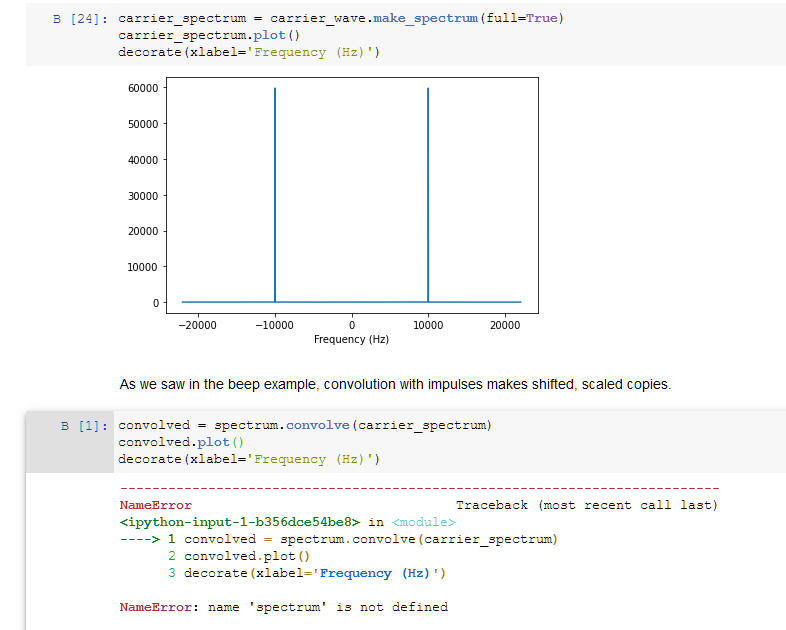
\includegraphics[width=0.75\textwidth]{images/ex1_dangerous.png}
        \caption{Опасное место}
        \label{fig:ex1_dangerous}
    \end{figure}
    
    Все ячейки выше работают нормально, а при запуске этой в консоли летят ошибки. 
    
    \begin{figure}[H]
        \centering
        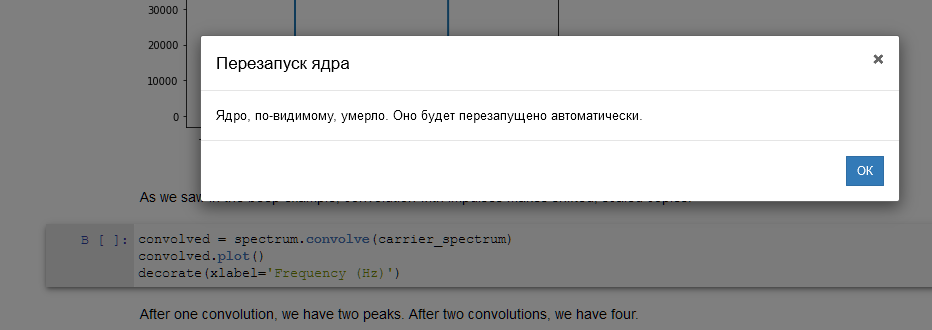
\includegraphics[width=0.75\textwidth]{images/ex1_error.png}
        \caption{Ошибка}
        \label{fig:ex1_error}
    \end{figure}
    
    Попробую сменить ядро \textquote{Python 3} на \textquote{Python 3.8.1 64-bit}... неа, не помогает. 
    
    Попробуем заменить в реализации \texttt{convolve()} версию \texttt{numpy} на \texttt{scipy}:
    
\begin{lstlisting}[language=Python,caption=Замена]
from thinkdsp import Spectrum

import scipy.signal

def convolve2(self, other):
    assert all(self.fs == other.fs)
    
    if self.full:
        hs1 = np.fft.fftshift(self.hs)
        hs2 = np.fft.fftshift(other.hs)
        hs = scipy.signal.fftconvolve(hs1, hs2, mode='same')
        hs = np.fft.ifftshift(hs)

    return Spectrum(hs, self.fs, self.framerate, self.full)

convolved = convolve2(spectrum, carrier_spectrum)
convolved.plot()
decorate(xlabel='Frequency (Hz)')
\end{lstlisting}

    Да, так работает! Придется везде внизу переписывать реализацию тогда.
    
    \chapter{Видеоролик}
    
    В этом задании нам предложено посмотреть: \sloppy{\texttt{https://youtu.be/cIQ9IXSUzuM}}. Вообще, выглядит вполне как достойный контент, а больше всего меня заинтересовал неплоский dithering, который еще и приглушить можно так, что мои уши уже будут неспособны воспринять его.
    
    \chapter{Импорты}
    
    \textquote{Полезные штуки} на все случаи жизни.
    
\begin{lstlisting}[language=Python,caption=Импорты]
from thinkdsp import Signal, Sinusoid, SquareSignal, TriangleSignal, SawtoothSignal, ParabolicSignal
from thinkdsp import normalize, unbias, PI2, decorate
from thinkdsp import Chirp
from thinkdsp import read_wave
from thinkdsp import Spectrum, Wave, UncorrelatedGaussianNoise, Spectrogram
from thinkdsp import Noise
from thinkdsp import CubicSignal
from thinkdsp import zero_pad

import numpy as np
import pandas as pd

from matplotlib import pyplot as plt

import thinkstats2

from scipy.stats import linregress

import scipy
import scipy.fftpack

import scipy.signal

from ipywidgets import interact, interactive, fixed
import ipywidgets as widgets

loglog = dict(xscale='log', yscale='log')

PI2 = np.pi * 2
\end{lstlisting}

    \chapter{Боремся со спектральными копиями}
    
    Наша задача теперь - сымитировать сэмплирование, из-за чего появятся спектральные копии (ведь это же воздействие последовательностью импульсов), а затем избавиться от этих копий при помощи \texttt{low\_pass()}, потому что они появятся в предсказуемых местах.

\begin{lstlisting}[language=Python,caption=Ударные]
wave = read_wave('Sounds/263868__kevcio__amen-break-a-160-bpm.wav')
wave.normalize()
wave.plot()
wave.make_audio()
\end{lstlisting}

    \begin{figure}[H]
        \centering
        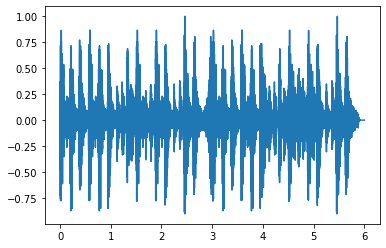
\includegraphics[width=0.75\textwidth]{images/ex2_drums.png}
        \caption{Исходный сигнал}
        \label{fig:ex2_drums}
    \end{figure}
    
    Этот сигнал будет как бы \textquote{настоящим} звуком. 
    
    Вот его спектр.
    
\begin{lstlisting}[language=Python,caption=Спектр]
spectrum = wave.make_spectrum(full=True)
spectrum.plot()
\end{lstlisting}

    \begin{figure}[H]
        \centering
        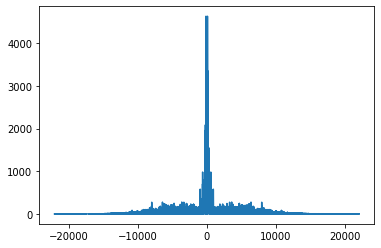
\includegraphics[width=0.75\textwidth]{images/ex2_spectrum.png}
        \caption{Настоящий спектр}
        \label{fig:ex2_spectrum}
    \end{figure}

    Сначала просто обрежем спектр:

\begin{lstlisting}[language=Python,caption=Сокращенный спектр]
factor = 5
framerate = wave.framerate / factor
cutoff = framerate / 2 - 1

spectrum.low_pass(cutoff)
spectrum.plot()

filtered = spectrum.make_wave()
filtered.make_audio()
\end{lstlisting}

    \begin{figure}[H]
        \centering
        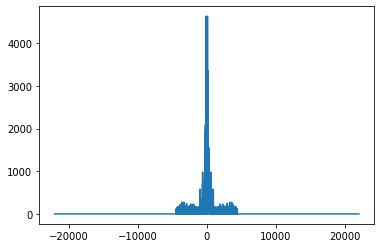
\includegraphics[width=0.75\textwidth]{images/ex2_filtered.png}
        \caption{Сокращенный Спектр}
        \label{fig:ex2_filtered}
    \end{figure}

    Теперь проведем симуляцию сэмплирования.
    
\begin{lstlisting}[language=Python,caption=Сэмплирование]
def sample(wave, factor):
    """Simulates sampling of a wave.
    
    wave: Wave object
    factor: ratio of the new framerate to the original
    """
    ys = np.zeros(len(wave))
    ys[::factor] = np.real(wave.ys[::factor])
    return Wave(ys, framerate=wave.framerate) 

sampled = sample(filtered, factor)

sampled_spectrum = sampled.make_spectrum(full=True)
sampled_spectrum.plot()

sampled.make_audio()
\end{lstlisting}

    \begin{figure}[H]
        \centering
        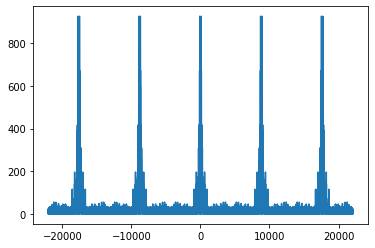
\includegraphics[width=0.75\textwidth]{images/ex2_sampled.png}
        \caption{Спектр результата сэмплирования}
        \label{fig:ex2_sampled}
    \end{figure}

    Обрежем его теперь по аналогии с тем, как мы это делали в первый раз и сравним с прошлым вариантом.
    
\begin{lstlisting}[language=Python,caption=Подчищаем спектр]
sampled_spectrum.low_pass(cutoff)
sampled_spectrum.scale(factor)
spectrum.plot()
sampled_spectrum.plot()
\end{lstlisting}

    \begin{figure}[H]
        \centering
        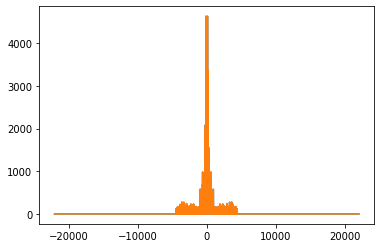
\includegraphics[width=0.75\textwidth]{images/ex2_fixed.png}
        \caption{Сравнение}
        \label{fig:ex2_fixed}
    \end{figure}

    Они не только выглядят идентично, но и звучат одинаково.

    % \printbibliography
    
\end{document}
